\documentclass{beamer}
\usepackage{ctex} %注意这个宏包
\usepackage{color}
\usepackage{graphics,graphicx}
\usepackage{pstricks,pst-node,pst-tree}
\usetheme{AnnArbor}
\usepackage{pstricks}
\usepackage{pst-plot}
\CTEXoptions[today=old]

\title{SQLAlchemy\\ Introduction and Promotion}
\author{严春伟}
\institute[PKUSZ]{
    互联网研发中心\\
}
\date{\today}

\begin{document}
% ------------- title page ----------------------------
%--- the titlepage frame -------------------------%
\begin{frame}
  \titlepage
\end{frame}

\section{Begin}
\begin{frame}
\frametitle{Outline}
\tableofcontents
\end{frame}

\section{Introduction}
\begin{frame}
\frametitle{Introduction}
\begin{block}{SQLAlchemy}
\begin{itemize}
    \item 一个开源的企业级的数据库ORM库
    \item 构成
    \begin{enumerate}
        \item SQL Toolkit
        \item Object Relational Mapper(ORM)
    \end{enumerate}
\end{itemize}
\end{block}

\begin{block}{类似的库}
    \begin{enumerate}
        \item Hiberate\quad Java
        \item Ruby on rails
    \end{enumerate}
\end{block}
\end{frame}

\begin{frame}{Organizations using SQLAlchemy}
    
\includegraphics[height=20pt]{oop_image/openstack.png}\\
    
\includegraphics[height=20pt]{oop_image/dropbox.png}\\
    
\includegraphics[height=20pt]{oop_image/firefox.png}\\
    
\includegraphics[height=20pt]{oop_image/fedora-logo.png}\\
    
\includegraphics[height=20pt]{oop_image/reddit.png}\\
\end{frame}

\begin{frame}{特点}
\begin{block}{优点}

\end{block}

\begin{block}{缺点}
\end{block}

\end{frame}

\section{Structure}

\begin{frame}{Structure}
    \begin{center}
    \frametitle{Structure}
    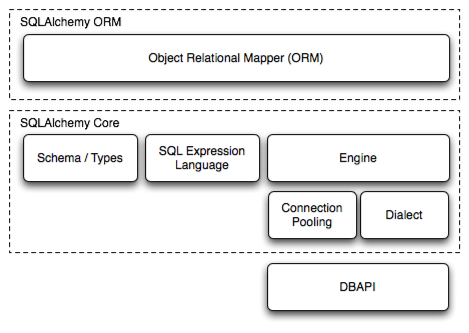
\includegraphics[height=140pt]{oop_image/structure.png}
    \end{center}
\end{frame}

\begin{frame}{Structure}
\begin{block}{Core}
\begin{itemize}
\item SQL语言扩充的工具箱
\item 有限的抽象
\end{itemize}

\end{block}
\begin{block}{ORM}
\begin{itemize}
\item 连接用户定义的类(class)和数据库中的表(table),实例(statement)和表中的行(row)
\item 透明地维持内存中对象和数据库中数据的一致性
\item 传达用户的数据库查询(query),包括类及关系
\end{itemize}
\end{block}
\end{frame}

\section{Core}
\begin{frame}{Core}
\begin{block}{Define and Create Table}
\begin{center}
\begin{columns}
%-- column one --
\begin{column}{4cm}
    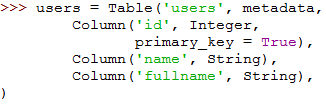
\includegraphics[height=50pt]{oop_image/core_table.png}
\end{column}

%-- column one --
\begin{column}{5cm}
    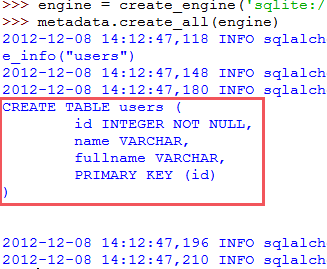
\includegraphics[height=100pt]{oop_image/sql_table.png}
\end{column}
\end{columns}
\end{center}
\end{block}
\end{frame}

%---- overprints --------
\begin{frame}{Core}
\begin{block}{Selecting}
\begin{center}
    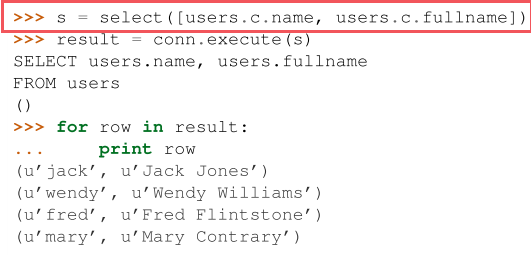
\includegraphics[height=100pt]{oop_image/core_select1.png}
\end{center}
\end{block}
\end{frame}

\begin{frame}{Core}
\begin{block}{Selecting}
\begin{center}
    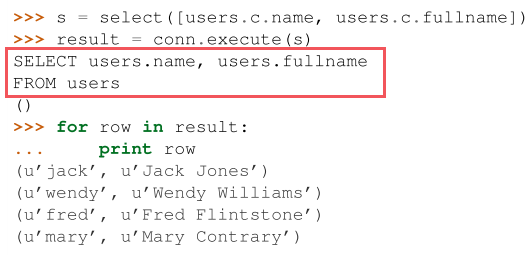
\includegraphics[height=100pt]{oop_image/core_select2.png}
\end{center}
\end{block}
\end{frame}
\begin{frame}{Core}
\begin{block}{Selecting}
\begin{center}
    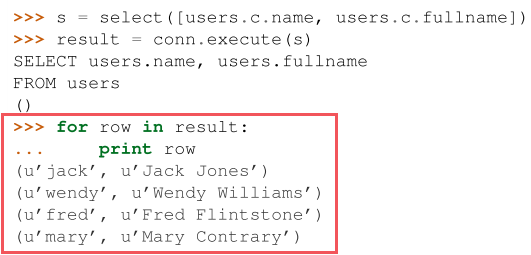
\includegraphics[height=100pt]{oop_image/core_select3.png}
\end{center}
\end{block}
\end{frame}

\begin{frame}{Core}
\begin{block}{总结}
\begin{enumerate}
    \item 函数级
    \item 一定程度的抽象
    \item 与底层SQL紧密联系
\end{enumerate}
\end{block}
\end{frame}

\section{ORM}
\begin{frame}
    \frametitle{ORM}
\begin{block}{Object Relational Mapper}
\begin{itemize}
\item 面向对象的抽象层
\item 基于Core层
\item 对表结构及操作的抽象
\end{itemize}
\end{block}
\end{frame}

\section{Expansion}





\end{document}
